\documentclass{article}
\usepackage{amsmath} % for advanced math environments
\usepackage{amsfonts} % for math fonts
\usepackage{amssymb} % for math symbols
\usepackage{amsthm} % for theorems and proofs
\usepackage{mathtools} % for mathematical tools
\usepackage{mathrsfs} % for script-like fonts in math
\usepackage{bm} % for bold math symbols
\usepackage{bbm} % for "blackboard-style" characters in math
\usepackage{graphicx} % for including graphics
\usepackage{hyperref} % for including hyperlinks
\usepackage{tcolorbox}
\tcbuselibrary{theorems, breakable}
\usepackage{xcolor}

\newcommand{\C}{\mathbb{C}}
\newcommand{\N}{\mathbb{N}}
\newcommand{\Q}{\mathbb{Q}}
\newcommand{\R}{\mathbb{R}}
\newcommand{\Z}{\mathbb{Z}}
\DeclareMathOperator{\lcm}{lcm}

\newtcolorbox[auto counter]{problem}%
{
    breakable,
    colback=cyan!5,
    colframe=cyan!35!black,
    fonttitle=\bfseries,
    title=Problem~\thetcbcounter,
}

\newtcolorbox{solution}[1]
{
    breakable,
    colback=red!5,
    colframe=red!75!black,
    fonttitle=\bfseries,
    title=Solution: #1,
}
\usepackage{tikz}
\usetikzlibrary{positioning}

% Title
\title{Your Document Title}
\author{Your Name}
\date{\today} % or specify a date like {December 2020}

\begin{document}

\maketitle

\section{Laws of Composition}

\section{Groups and Subgroups}

\section{Subgroups and the Additive Group of Integers}


\begin{problem}
Let $a = 123$ and $b = 321$. Compute $d = \gcd(a, b)$, and express $d$ as an integer combination $ra + sb$.
\end{problem}

\textbf{Solution: use the Euclidean algorithm}.
\\

Since $a$ is the smaller number we'll write $b$ as $qa + r$. Using the Euclidean algorithm:
\begin{align*}
    321 & = 2 \cdot 123 + 75 \\
    123 & = 1 \cdot 75 + 48  \\
    75  & = 1 \cdot 48 + 27  \\
    48  & = 1 \cdot 27 + 21  \\
    27  & = 1 \cdot 21 + 6   \\
    21  & = 3 \cdot 6 + 3    \\
    6   & = 2 \cdot 3 + 0
\end{align*}
which shows that 3 is the greatest common denominator. To find the integer combination, start with the last equation with remainder, $21 = 3(6) + 3$. Solving for the remainder gives $3 = 21 - 3(6)$. Work backwards, substituting the lower remainder in each line and combining like terms:
\begin{align*}
    3 & = 21 - 3(6)                  & \text{last eqation with remainder} \\
      & = 21 - 3(27 - 21)            & \text{substitute}                  \\
      & = 4(21) - 3(27)              & \text{combine like terms}          \\
      & = 4(48 - 27) - 3(27)         & \text{substitute}                  \\
      & = 4(48) - 7(27)              & \text{combine like terms}          \\
      & = 4(48) - 7(75 - 48)         & \text{substitute}                  \\
      & = 11(48) - 7(75)             & \text{combine like terms}          \\
      & = 11(123 - 75) - 7(75)       & \text{substitute}                  \\
      & = 11(123) - 18(75)           & \text{combine like terms}          \\
      & = 11(123) - 18(321 - 2(123)) & \text{substitute}                  \\
      & = 47(123) - 18(321)          & \text{combine like terms}
\end{align*}
Therefore $d = 3$ and $3 = 47(123) - 18(321)$.

\begin{problem}
Prove that if $a$ and $b$ are positive integers whose sum is a prime $p$, their greatest common divisor is 1.
\end{problem}
\textbf{Proof: use direct proof}.
\\

Let $\gcd(a, b) = d$. Then $d$ divides $a$ and $b$, so $d$ divides $a + b = p$. Since $p$ has no divisors other than itself and 1, it must be that $d = 1$. It cannot be $d = p$ since $p > a, b$.

\begin{problem}
\textbf{(a)} Define the greatest common divisor of a set $\{a_1, \ldots, a_n\}$ of $n$ integers. Prove it exists, and that it is an integer combination of $a_1, \ldots, a_n$.
\textbf{(b)} Prove that if the greatest common divisor of $\{a_1, \ldots, a_n\}$ is $d$, then the the greatest common divisor of $\{a_1 / d, \ldots, a_n / d\}$ is 1.
\end{problem}

\textbf{(a) Proof: fundamental theorem of arithmetic}. Define the gcd of $n$ integers as the greatest positive divisor for all $n$ integers. Since 1 divides every integer, the gcd exists and is always at least 1. View each number by its prime decomposition, and the gcd defined here is the product of primes with each prime's exponent the minimum of the exponents on the same primes among the $a_i$'s.

Base case: using prime decomposition, the gcd of any two integers is the product of primes with the lower of the two exponents on each prime. For example:
$$a = p_1^{e_1} p_2^{e_2} \ldots p_k^{e_k} \quad b = p_1^{f_1} p_2^{f_2} \ldots p_k^{f_k}$$
would have:
$$\gcd(a, b) = p_1^{\min(e_1, f_1)} p_2^{\min(e_2, f_2)} \ldots p_k^{\min(e_k, f_k)}$$

For the inductive hypothesis, assume $d = \gcd(a_1, \ldots, a_{n-1})$ and each $a_i$ has prime decomp exponents $e_{1_i}, e_{2_i}, \ldots$. Then $d$ is the product of primes where the exponent on the $j$th prime is the minimum of the exponents of the $j$th prime among the $a_i$'s:
$$p_j^{\min(e_{j_1}, e_{j_2}, \ldots, e_{j_{n-1}})}$$

Now for the inductive step. It must be by definition that $e = \gcd(a_1, \ldots, a_n)$ has a prime decomposition where the exponent on the $j$th prime is again the minimum exponent on the $j$th prime across $a_1$ through $a_n$:
$$p_j^{\min(e_{j_1}, e_{j_2}, \ldots, e_{j_n})}$$

This also shows us that $e = \gcd(d, a_n)$, since we can equivalently compute $e$ by first taking the minimum prime exponents on the first $n-1$ numbers, then taking the minimum of that with $a_n$'s prime exponents or taking the min of all at once. By the inductive hypothesis and base case, we can write:
$$e = dx + ya_n, \quad d = \sum_{i=1}^{n-1} q_i a_i \implies e = xq_1 a_1 + \ldots xq_{n-1}a_{n-1} + ya_n$$

\section{Cyclic Groups}
\makeatletter
\setcounter{tcb@cnt@problem}{0}
\makeatother
\begin{problem}
Let $a$ and $b$ be elements of a group $G$. Assume that $a$ has order 7 and that $a^3b = ba^3$. Prove that $ab = ba$.
\end{problem}
\textbf{Proof: use algebra}
\\

Since $a^7 = 1$ we can write $a = a^7a^7a$. Using this and regrouping to get factors of $a^3 b$ we can rewrite them as $ba^3$ to commute the $a$'s past the $b$:
\begin{align*}
    ab & = a^{15}b        & a^{15} = a^7 a^7 a \\
       & = a^{12}a^{3}b   &                    \\
       & = a^{12}ba^{3}   & ab^3 = ba^3        \\
       & = a^{9}a^{3}ba^3 &                    \\
       & = a^{9}ba^{6}    &                    \\
       & = a^6 a^3 b a^6  &                    \\
       & = a^6 ba^9       &                    \\
       & = a^3 ba^{12}    &                    \\
       & = ba^{15}        &                    \\
       & = ba             &                    \\
\end{align*}

\begin{problem}
An $n$ root of unity is a complex number $z$ such that $z^n = 1$.
\\
\textbf{(a)} Prove that the $n$ roots of unity form a cyclic subgroup of $\C^\times$ of order $n$.
\\
\textbf{(b)} Determine the product of all $n$th roots of unity.
\end{problem}
\textbf{(a) Proof: use algebra}
\\

Suppose $z$ is a complex number and an $n$th root of unity. Therefore $z^n = 1$. The $n$ roots of unity are $\{z^0, z^1, \ldots, z^{n-1}\}$ and we must prove this is a cyclic subgroup of order $n$. First, it contains the identity 1 since $z^0 = 1$. Second, suppose $k, \ell$ are powers of $z$ in the set. Then $z^k z^\ell = z^{k + \ell}$. If $k + \ell < n$ then $z^{k + \ell}$ is in the set. If $k + \ell \geq n$ then $k + \ell = n + r$ for some $0 \leq r < n$. In that case $z^{k + \ell} = z^{n+r}=z^n z^r = z^r$, which is in the set. Therefore the set is closed under composition. To show inverses, any $k \in \{1, \ldots, n-1\}$ has a complementary number $\ell$ in $\{1, \ldots, n-1\}$ that sums to $n$, giving $z^k z^\ell = z^{k + \ell} = z^n = 1$. Therefore roots of unity are closed under inversion and they form a subgroup of $\C^\times$. There are $n$ elements in the set, so it has order $n$.
\\

\textbf{(b) Proof: consider the cancellation from inverses}
\\

The product of all roots of unity are $z^0 z^1 \ldots z^{n-1}$. If $n$ is odd then for each $z^k$ there is a $z^{n-k}$ inverting it and the product will be 1. If $n$ is even then $z^{n/2}$ is its own inverse and every other elements will have a distinct inverse. Therefore the product of all roots will simplify to $z^{n/2}$. Here $z^0 \neq z^{n/2}$, meaning $z^{n/2}$ is not 1 but when multiplied by itself becomes 1. This requires that $z^{n/2} = -1$.

So in general, the product of all $n$th roots will be 1 if $n$ is odd and -1 if $n$ is even, or $(-1)^{n+1}$.

\begin{problem}
Let $a$ and $b$ be elements of a group $G$. Prove that $ab$ and $ba$ have the same order.
\end{problem}

\textbf{Proof: use algebra}
\\

Assuming this is a finite group, all elements have finite order. Suppose $\text{ord}(ab) = k$. Then
$$(ab)^k = abab\ldots ab \quad \text{($k$ times)} = 1$$

Multiply by $a^{-1}$ on the left and $b^{-1}$ on the right to get:
$$baba\ldots ba \quad \text{($k-1$ times)} = (ba)^{k-1} = a^{-1}b^{-1} = (ba)^{-1}$$

Now multiplying both sides by $ba$ gives $(ba)^k = 1$. Therefore $\text{ord}(ba) = k$ as well.

\begin{problem}
Describe all groups $G$ that have no proper subgroup.
\end{problem}
There is the trivial group whose only subgroup is itself. There is also $\Z_2$ whose only subgroups are itself and the trivial group. Beyond that, any cyclic group with even order $2k$ has a proper subgroup containing an element of order $k$ and the identity. Indeed for a group of any size, if it contains elements besides $e$ that have an order dividing the order of the group, the subgroup generated by that element becomes a proper subgroup.

Next we eliminate infinite groups: suppose $G$ is infinite and has an infinite order element $x$. Then $\langle x \rangle$ forms a subgroup equivalent to the integers $(x^k \cong k)$. Next, suppose that $G$ is infinite and contains a finite order element besides the identity. Then there exists an $x \in G$ such that $x^k = e$ for some $k$, which means $\langle x \rangle$ is a proper subgroup, a cyclic group of order $k$. Since an infinite $G$ with infinite order members or finite order members contain proper subgroups, no infinite order group lacks a proper subgroup.

The only remaining case are finite groups of odd order with no divisors: in other words we consider groups with prime order $p > 2$. The order of any non-identity element $x$ must be relatively prime to the order of the group: for $x^k$, $k$ and $p$ cannot have any common factors larger than 1 since $p$ is prime. This requires the order of $x^k$ to be $p$ for all $k$, which means that any $x^k$ generates the group. Therefore prime order groups contain no proper subgroups.

\begin{problem}
Prove that every subgroup of a cyclic group is cyclic. Do this by working with exponents and use the description of the subgroups of $\Z^+$.
\end{problem}

\textbf{Proof: relate to the additive integers group}
\\

Suppose group $C$ is cyclic and has subgroup $H$ generated by $x^{k_1}, \ldots, x^{k_n}$. A group with such generators functions as $\Z k_1 + \ldots + \Z k_n$ which is always equivalent to $\Z d$ where $d = \gcd(k_1, \ldots, k_n)$. Therefore we can say $H = \langle x^d \rangle$ and is cyclic.

\begin{problem}
\textbf{(a)} Let G by a cyclic group of order 6. How many of its elements generate $G$? Answer the same question for cyclic groups of orders 5 and 8.

\textbf{(b)} Describe the number of elements that generate a cyclic group of arbitrary order $n$.
\end{problem}
\textbf{(a) Proof: analyze the element orders}
\\
Write the cyclic group of order 6 as $\{e, x, x^2, x^3, x^4, x^5\}$. We want to find the elements with an order $k$ whose least common multiple with 6 is $6k$. That would mean $x^k$ must be composed with itself 6 times to become $e$, and $\langle x^k \rangle$ would have order 6. The elements that fit this description will have exponents relatively prime to 6, which are 1 and 5. Therefore $\langle x \rangle$ and $\langle x^5 \rangle$ can generate $G$.
\\

By the rule that any cylic group element with order relatively prime to the group order will generate the group, we can see that any non-identity element of $C_5$ will generate the group (or note that this is a prime order group and use the result from above). For $C_8$ the elements that can generate it are $x, x^3, x^5, x^7$.

\textbf{(b) Proof: use arithmetic}
\\

We have established the rule that in a cyclic group order $n$, any element with an order relatively prime to $n$ will generate the group.

\begin{problem}
Let $x$ and $y$ be elements of group $G$. Assume that each of the elements $x, y$, and $xy$ has order 2. Prove that the set $H = \{1, x, y, xy\}$ is a subgroup of $G$ and that it has order 4.
\end{problem}

\textbf{Proof: directly prove $H$ has each property required}
\\

First we'll show that $H$ is a subgroup of $G$. It contains the identity $1$. For closure under composition, note that $x, y$ and $xy$ all have order 2 which is another way of saying they are their own inverses, so we have closure under inversion. The only composition that could be missing is $yx$ but we can show that in fact $yx = xy$. We can write $(xy)^{-1} = y^{-1} x^{-1} = yx$, but since $xy$ has order 2 it is also the case that $(xy)^{-1} = xy$. This implies that $xy = yx$ and $H$ is closed under composition. So $H$ satisfies all the properties of a group with 4 members, making it order 4.

\begin{problem}
\textbf{(a)} Prove that the elementary matrices of the first and third types (1.2.4) generate $GL_n(\R)$.

\textbf{(b)} Prove that the elementary matrices of the first type generate $SL_n(\R)$.
\end{problem}
\textbf{(a) Proof: }
\\

The `first type' elementary matrix is an identity matrix with one non-zero entry somewhere off the diagonal. Suppose matrix $E_1$ has value $a$ at index $(i, j)$, then when $E$ multiplies a matrix $B$, matrix $E$ adds $a$ times the $jth$ row in $B$ to the $i$th row in the product $EB$.

The `third type' elementary matrix is an identity but with one of the diagonal entries replaced by a value $a \neq 1$ (and non-zero). This has the effect of multiplying the $i$th row in its product by $a$.

If we are trying to generate $GL_n(\R)$, only these two types are needed. The `second type' of elementary matrix swaps rows, which is not necessary here since we can build up any invertible matrix by composing types one and three.

To generate any $B \in GL_n(\R)$ from these elementary matrices, first build the diagonal: for each entry $b_{ii}$ on $B$'s diagonal use a type 3 elementary matrix with $b_{ii}$ at index $(i,i)$. Composing these together will give the digaonal of $B$:
$$\begin{bmatrix}b_{11} & & & \\ & 1  & & \\ & & \ddots & \\ & & & 1\end{bmatrix}
    \begin{bmatrix}1 & & & \\ & b_{22}  & & \\ & & \ddots & \\ & & & 1\end{bmatrix}
    \ldots
    \begin{bmatrix}1 & & & \\ &1  & & \\ & & \ddots & \\ & & & b_{nn}\end{bmatrix}
    = \begin{bmatrix}b_{11} & & & \\ & b_{22}  & & \\ & & \ddots & \\ & & & b_{nn}\end{bmatrix}$$

Then for any off-diagonal entry $b_{ij}$, use a type 1 elementary matrix with $b_{ij} / b_{ii}$ at index $(i,j)$, and 1's on the diagonal. Composing these together will give the off-diagonal entries of $B$:
$$\begin{bmatrix}1 & b_{12} / b_{11} & \ldots & \\ b_{21} / b_{22} & 1  & & \\ \vdots & & 1 & \\ & & & 1\end{bmatrix}$$

Multiplying this on the left by the diagonal matrix gives $B$: by the row picture of matrix multiplication, the first row in the product becomes the vector $b_{11}(1, b_{12} / b_{11}, b_{13} / b_{11}, \ldots , b_{1n} / b_{11}) = (b_{11}, b_{12}, b_{13}, \ldots, b_{1n})$. Continuing this way for each row we get $b_{ij}$ in the product matches $b_{ij}$ in $B$. Therefore, these elementary matrices can produce any matrix in $GL_n(\R)$ and generate the group.
\\

\textbf{(b) Proof: use determinant properties.}
\\

The type 1 matrices all have determinant 1, so composing them will always give a matrix in $SL_n(\R)$. Mutliplying by a type 3 matrix would necessarily change the determinant so they cannot be used to produce a matrix in $SL_n(\R)$. Therefore type 1 matrices suffice to generate $SL_n(\R)$.

\begin{problem}
How many elements of order 2 does the symmetric group $S_4$ have?
\end{problem}

\textbf{Proof: look for alternative views of order 2 elements}
\\

In a symmetric group, an order 2 element would be its own inverse. This would include transpositions, and in $S_4$ we have $\binom{4}{2}=6$ transpositions:
$$\{(12), (13), (14), (23), (24), (34)\}$$

But notice that the composition of two disjoint transpositions would also have order 2. Verify this by composing two disjoint transpositions with itself, such as $((12)(34))^2$:
\begin{center}
    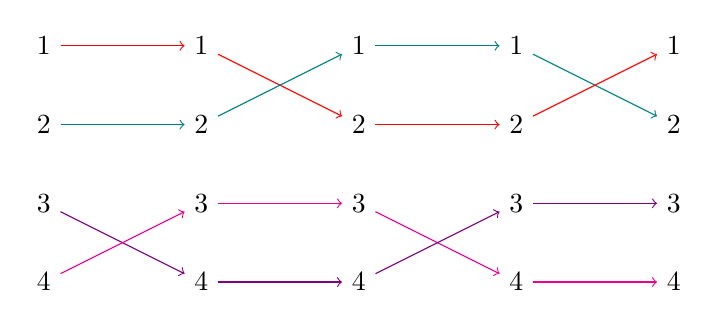
\begin{tikzpicture}[node distance=1cm, auto]
        \node (n1) {1};
        \node (n2) [below of=n1] {2};
        \node (n3) [below of=n2] {3};
        \node (n4) [below of=n3] {4};

        \node (m1) [right of=n1, node distance=2cm] {1};
        \node (m2) [below of=m1] {2};
        \node (m3) [below of=m2] {3};
        \node (m4) [below of=m3] {4};



        \node (p1) [right of=m1, node distance=2cm] {1};
        \node (p2) [below of=p1] {2};
        \node (p3) [below of=p2] {3};
        \node (p4) [below of=p3] {4};

        \node (q1) [right of=p1, node distance=2cm] {1};
        \node (q2) [below of=q1] {2};
        \node (q3) [below of=q2] {3};
        \node (q4) [below of=q3] {4};

        \node (r1) [right of=q1, node distance=2cm] {1};
        \node (r2) [below of=r1] {2};
        \node (r3) [below of=r2] {3};
        \node (r4) [below of=r3] {4};

        \draw[->, draw=red] (n1) -- (m1);
        \draw[->, draw=teal] (n2) -- (m2);
        \draw[->, draw=violet] (n3) -- (m4);
        \draw[->, draw=magenta] (n4) -- (m3);

        \draw[->, draw=red] (m1) -- (p2);
        \draw[->, draw=teal] (m2) -- (p1);
        \draw[->, draw=magenta] (m3) -- (p3);
        \draw[->, draw=violet] (m4) -- (p4);

        \draw[->, draw=teal] (p1) -- (q1);
        \draw[->, draw=red] (p2) -- (q2);
        \draw[->, draw=magenta] (p3) -- (q4);
        \draw[->, draw=violet] (p4) -- (q3);

        \draw[->, draw=teal] (q1) -- (r2);
        \draw[->, draw=red] (q2) -- (r1);
        \draw[->, draw=violet] (q3) -- (r3);
        \draw[->, draw=magenta] (q4) -- (r4);
    \end{tikzpicture}
\end{center}

So in $S_4$ we have 6 individual transpositions plus 3 disjoint transposition products, $(12)(34), (13)(24)$ and $(14)(23)$, for a total of 9 order 2 elements.

\begin{problem}
Show by example that the product of elements of finite order in a group need not have finite order. What if the group is abelian?
\end{problem}

\textbf{Solution:}

To find such an example we must look in infinite groups since in any finite group the product of two members with finite order will be the lcm of their individual orders.

Consider the group of permutations on the integers under addition. The permutations $f(x) = -x$  and $g(x) = -x + 1$ both have order 2. However their composition $g(f(x)) = -(-x + 1) = x - 1$ has infinite order.

\begin{problem}
\textbf{(a)} Adapt the method of row reduction to prove that the transpositions generate the symmetric group $S_n$.

\textbf{(b)} Prove that, for $n \geq 3$, the three-cycles generate the alternating group $A_n$.

\end{problem}

\textbf{(a) Proof:} Take a matrix with $n$ rows and consider them the letters 1 through $n$. The elementary matrix that swaps rows $i$ and $j$ corresponds to the transposition $(ij)$. Since any ordering of the matrix' rows is possible by composing these elementary matrices, we can construct any permutation of $n$ letters by the same corresponding transpositions. Therefore the transpositions generate $S_n$.

\textbf{(b) Proof: show mutual inclusion} Any permutation in $A_n$ must be even which means it decomposes to an even number of transpositions $(ab)(cd)\ldots(wx)(yz)$. For any consecutive transposition pair $(ab)(cd)$ separate into three cases and show that each one can be written as a product of three-cycles:
\begin{enumerate}
    \item $(ab)$ and $(cd)$ share two letters, that is $(ab) = (cd)$
    \item $(ab)$ and $(cd)$ share one letter (either $a = c$ or $b = d$, but not both)
    \item $(ab)$ and $(cd)$ have no letters in common
\end{enumerate}

For the first case $(ab)(cd) = (ab)(ab) = 1$ and therefore can be removed from the product (or expressed as any $(ijk)^3$ for any distinct $i, j, k$).

For the second case, assume WLOG that $b = c$ so $(ab)(cd) = (ab)(bd) = (abd)$:
\begin{center}
    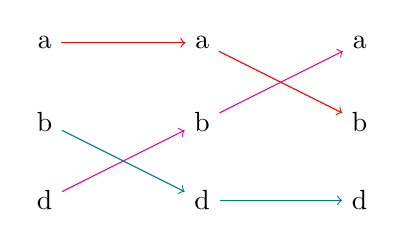
\begin{tikzpicture}[node distance=1cm, auto]
        \node (n1) {a};
        \node (n2) [below of=n1] {b};
        \node (n3) [below of=n2] {d};

        \node (m1) [right of=n1, node distance=2cm] {a};
        \node (m2) [below of=m1] {b};
        \node (m3) [below of=m2] {d};

        \node (p1) [right of=m1, node distance=2cm] {a};
        \node (p2) [below of=p1] {b};
        \node (p3) [below of=p2] {d};

        \draw[->, draw=red] (n1) -- (m1);
        \draw[->, draw=magenta] (n3) -- (m2);
        \draw[->, draw=teal] (n2) -- (m3);

        \draw[->, draw=red] (m1) -- (p2);
        \draw[->, draw=magenta] (m2) -- (p1);
        \draw[->, draw=teal] (m3) -- (p3);

    \end{tikzpicture}
\end{center}

For the third case, $(ab)(cd)$ can be written as $(abc)(abd)$:
\begin{center}
    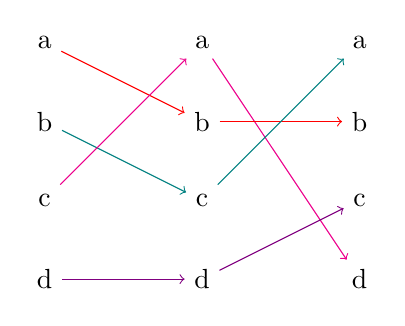
\begin{tikzpicture}[node distance=1cm, auto]
        \node (n1) {a};
        \node (n2) [below of=n1] {b};
        \node (n3) [below of=n2] {c};
        \node (n4) [below of=n3] {d};

        \node (m1) [right of=n1, node distance=2cm] {a};
        \node (m2) [below of=m1] {b};
        \node (m3) [below of=m2] {c};
        \node (m4) [below of=m3] {d};

        \node (p1) [right of=m1, node distance=2cm] {a};
        \node (p2) [below of=p1] {b};
        \node (p3) [below of=p2] {c};
        \node (p4) [below of=p3] {d};

        \draw[->, draw=red] (n1) -- (m2);
        \draw[->, draw=teal] (n2) -- (m3);
        \draw[->, draw=magenta] (n3) -- (m1);
        \draw[->, draw=violet] (n4) -- (m4);

        \draw[->, draw=magenta] (m1) -- (p4);
        \draw[->, draw=red] (m2) -- (p2);
        \draw[->, draw=teal] (m3) -- (p1);
        \draw[->, draw=violet] (m4) -- (p3);

    \end{tikzpicture}
\end{center}
Therefore, three-cycles can generate any even permutation and $A_n \subseteq \langle \text{3-cycles} \rangle$.

To prove $\langle \text{3-cycles} \rangle \subseteq A_n$ notice that any $(abc) = (ab)(bc)$, a product of two transpositions and therefore even. Any product of three-cycles then decomposes into pairs of transpositions, and these products will also be even. Therefore $\langle \text{3-cycles} \rangle \subseteq A_n$. Since we have shown that $A_n \subseteq \langle \text{3-cycles}\rangle$ we have $A_n = \langle \text{3-cycles} \rangle$.

\section{Homomorphisms}
\begin{problem}
Let $\varphi: G \to G'$ be a surjective homomorphism. Profve that if $G$ is cyclic, then $G'$ is cyclic, and if $G$ is abelian then $G'$ is abelian.
\end{problem}

\textbf{Proof: use the properties of homomorphisms}

Suppose $G$ is cyclic, then it's generated by a single element $g$ and any $G$ member equals $g^n$ for some $n$. Since $\varphi$ is homomorphic, $\varphi(g^n) = \varphi(g)^n$ which means the image $\varphi(G)$ can only reach powers of $\varphi(g)$. However, $\varphi$ is surjective which means these powers of $\varphi(g)$ can reach any $g' \in G'$. Therefore any member of $G'$ is a power of $\varphi(g)$ and we can say the single element $\varphi(g)$ generates $G'$, making it a cyclic group.
\\

Now suppose $G$ is abelian. Then for any $a, b \in G$ we have $ab = ba$ so $\varphi(ab) = \varphi(ba)$. This implies $\varphi(a)\varphi(b) = \varphi(b)\varphi(a)$. Since $\varphi$ can reach any $G'$ member, this commutativity applies to all $G'$ members showing that the group is abelian.

\begin{problem}
Prove that the intersection $K \cap H$ of subgroups of a group $G$ is a subgroup of $H$, and that if $K$ is a normal subgroup of $G$, then $K \cap H$ is a normal subgroup of $H$.
\end{problem}

\textbf{Proof: use the definition of subgroups and normal subgroups}

Suppose $K$ and $H$ are both subgroups of $G$. Then $1 \in K$ and $1 \in H$ making $1 \in K \cap H$, so the intersection contains the identity.

For inverses: any $g \in K \cap H$ we must have $g \in K$ and $g \in H$ as well. Since $K, H$ are subgroups they contain all inverses, so $g^{-1}$ is in both $K$ and $H$ as well, making $g^{-1}$ in the intersection. So $K \cap H$ contains all inverses.

For composition: suppose $g, h \in K \cap H$. Then both $g$ and $h$ are in $K$ and $H$, so $gh \in K$ and $gh \in H$ as well, making $gh \in K \cap H$. Therefore subgroup intersections are still subgroups.
\\

Now suppose $K$ is a normal subgroup of $G$, and contains every conjugate in $K$ by $G$, $gkg^{-1}$. Then certainly $K$ contains every conjugate by $H$, $hkh^{-1}$, since $H \leq G$. Now consider any $m \in K \cap H$. Since $m$ appears in the intersection it must be in $K$ as well, meaning $hmh^{-1} \in K$ for any $h \in H$ because $K$ is closed under conjugation. Also $m \in H$ because $m$ appears in the intersection, which implies $hmh^{-1} \in H$ since $H$ has closure. Therefore these conjugates will also be in the intersection $K \cap H$. Since $K \cap H$ contains all conjugates of its members by $H$, it is a normal subgroup of $H$.

\begin{problem}
Let $U$ denote the group of invertible upper triangular $2 \times 2$ matrices $A = \begin{bmatrix} a & b \\ 0 & d \end{bmatrix}$, and let $\varphi: U \to \R^\times$ be the map that sends $A \rightsquigarrow a^2$. Prove that $\varphi$ is a homomorphism, and determine its kernel and image.
\end{problem}

\textbf{Prove $\varphi$ is a homomorphism using algebra}
Let $B = \begin{bmatrix} e & f \\ 0 & h \end{bmatrix}$ be another invertible upper triangular matrix in $U$. Then $\varphi(A) = a^2$ and $\varphi(B) = e^2$. The matrix $AB$ has $ae$ in its upper left corner, so $\varphi(AB) = (ae)(ae)$. But since real multiplication commutes we have $(ae)(ae) = a^2 e^2 = \varphi(A)\varphi(B) = \varphi(AB)$, making $\varphi$ a homomorphism.

The kernel will be those matrices whose $a$ entry squared is 1. That means any matrix in $U$ whose $a = \pm 1$ will map to 1, the identity in $\R^\times$. For the image, consider all the possible values of $a^2$. This must be at least 0, but in fact for $a^2$ to equal 0 it would have to be $a = 0$, but that would make the matrix in $U$ uninvertible. So we can deduce that no matrix in $U$ has $a = 0$. Since $a^2$ can't be negative or 0, it must be positive. And any positive real number has a positive principal square root. This root can be a first entry in a $U$ matrix, therefore any $\varphi$ can reach any positive real number, making the image $\varphi(U) = \R^{>0}$.

\begin{problem}
Let $f: R^+ \to \C^\times$ be the map $f(x) = e^{ix}$. Prove that $f$ is a homomorphism, and determine its kernel and image.
\end{problem}

\textbf{Proof $f$ is a homomorphism using algebra}
\\

Given $f(x) = e^{ix}$ and $f(y) = e^{iy}$:
$$f(x+y) = e^{i(x+y)} = e^{ix + iy} = e^{ix}e^{iy} = f(x)f(y)$$

Therefore $f$ is a homomorphism.

\textbf{Find the kernel and image of $f$}
The kernel of $f$ will be those real numbers $x$ that make $e^{ix} = 1$. The only way for this to happen is if $x = 0$. Therefore $f$ has a trivial kernel. To find the image of $f$ it helps to recognize that $e^{ix}$ follows the Euler formula, an exponential view of complex numbers. In this view the coefficient on $e$ gives the radius and $x$ gives the angle. Since $f$ can map to any $x$ but in its image the coefficient is always 1, $f$'s image is all complex numbers with radius 1: the unit circle in $\C^\times$.

\begin{problem}
Prove that the $n \times n$ matrices that have the block form $M = \begin{bmatrix} A & B \\ 0 & D\end{bmatrix}$, with $A$ in $GL_r{\R}$ and $D$ in $GL_{n-r}(\R)$, form a subgroup $H$ of $GL_n(\R)$, and that the map $H \to GL_r(\R)$ that sends $M \rightsquigarrow A$ is a homomorphism. What is its kernel?
\end{problem}

\textbf{Proof $H$ is a subgroup by showing it has all subgroup properties.}
By forming the block matrix with $A = I_r, D = I_{n-r}$ and $B = 0$ we get the identity $I_n$, so $H$ contains the identity. For inverses, set up a product:
\[
    \begin{array}{cc}
                                   & \begin{bmatrix} E & F \\ 0 & G \end{bmatrix} \\
        \begin{bmatrix} A & B \\ 0 & D \end{bmatrix} & \begin{bmatrix} AE & AF + BG \\ 0 & DG \end{bmatrix}
    \end{array}
\]

We see here if we set $E = A^{-1}, G = D^{-1}$ then the block diagonal will be identities. We want $AF + BG = 0$ so the product is the identity in $GL_n(\R)$, so we can solve for $F$:
$$AF + BG = 0 \implies AF + BD^{-1} = 0 \implies F = -A^{-1}BD^{-1}$$

So the inverse of $\begin{bmatrix} A & B \\ 0 & D \end{bmatrix}$ is $\begin{bmatrix} A^{-1} & -A^{-1}BD^{-1} \\ 0 & D^{-1} \end{bmatrix}$, which has invertible matrices on the block diagonal and a 0 in the bottom left, making it a member of $H$.

To show closure under composition, consider blocks in the product matrix again: $AE$ and $DG$ are the products of invertible matrices and thus invertible themselves. $AF + BG$ is anything, and we have a 0 in the bottom left block. Therefore the product of any two matrices in $H$ follows the block form and is a member of $H$, and $H$ is a subgroup of $GL_n(\R)$.
\\

\textbf{Proof that $M \rightsquigarrow A$ is a homomorphism using algebra.}

Let $M = \begin{bmatrix} A & B \\ 0 & D \end{bmatrix}$ and $L = \begin{bmatrix} E & F \\ 0 & G \end{bmatrix}$. Call the map $\phi$ that projects a matrix in $H$ to its upper-left block: $\phi(M) = A$ and $\phi(L) = E$. Then $\phi(ML) = AE = \phi(M)\phi(L)$, so $\phi$ is a homomorphism.

\textbf{Find the kernel of $\phi$.}

By definition, $\phi$'s kernel are those matrices $M$ that become $I_r$ after projection. That happens only when $A = I_r$.

\begin{problem}
Determine the center of $GL_n(\R)$.
\\

\textit{Hint}: You are asked to determine the invertible matrices $A$ that commute with every invertible matrix $B$. Do not test with a general matrix $B$. Test with elementary matrices.
\end{problem}

By basic matrix properties, we know that $I$ commutes and $\lambda I$ for any $\lambda \in \R$ will also commute because the scalar $\lambda$ can factor out of any product: $(\lambda I)B = \lambda IB = B(\lambda I)$. So the center of $GL_n(\R)$ will contain all scalar multiples of the identity.

Following Artin's hint, we can actually show that no elementary matrices commute in general ($\lambda I$ is not an elemenatry matrix according to Artin's definition):

Type I matrices have 1's on the diagonal and one nonzero entry $a$ off the diagonal at some index $(i, j)$. This causes its operand to add $a$ times its $j$th row to its $i$th row. Here the order would matter: suppose we will add a multiple of row $j$ to row $k$, then a multiple of $i$ to row $j$. If we apply the row $i$ multiple to row $j$ first, then a different multiple gets added to row $k$. Therefore Type I matrices don't all commute with each other and can't be in the center.
\\

Type II matrices swap rows $i$ and $j$, much like transpositions in $S_n$. Consider the swaps $(ij)$ and $(jk)$. Then $(ij)(jk) = (ijk)$ but $(jk)(ij) = (ijk)$. So composition order matters here as well, and Type II matrices don't all commute with each other, leaving them out of the center.
\\

Type III matrices are all 1's on the diagonal except one diagonal entry will be $c \neq 0$. Suppose such a matrix $A$ has $c$ appearing at entry $(i, i)$, then its operand's $i$th row will be multiplied by $c$.  For another Type III matrix $B$ with $d$ at $(j, j)$, if $j = i$ then $AB$ has the effect of multiplying the operand's $i$th row by scalars $c$ then $d$. Scalar multiplication is commutative, so this is the same as multiplying by $d$ then $c$, and $AB = BA$. If $j \neq i$, then $B$ operates on a totally different row than $A$ and again the order won't matter, making $AB = BA$. Therefore Type III matrices commute with each other.
\\

The question remains if Type III matrices commute with Type I and II matrices. A quick check shows that they do not in general commute:
$$\begin{bmatrix}1 & a \\ 0 & 1 \end{bmatrix}\begin{bmatrix}c & 0 \\ 0 & 1\end{bmatrix} = \begin{bmatrix}c& a \\ 0 & 1\end{bmatrix}, \quad \begin{bmatrix}c & 0 \\ 0 & 1\end{bmatrix}\begin{bmatrix}1 & a \\ 0 & 1 \end{bmatrix} = \begin{bmatrix} c & ca \\ 0 & 1\end{bmatrix}$$

\section{Isomporphisms}
\begin{problem}
Let $G'$ be the group of real matrices of the form $\begin{bmatrix} 1 & x \\ & 1\end{bmatrix}$. Is the map $\R^+ \to G'$ that sends $x$ to this matrix an isomorphism?
\end{problem}

\textbf{Proof: show that the map is homomorphic and bijective.}
\\
Call this map $\phi$:
\begin{align*}
    \phi: \R^+ & \to G'                             \\
    x          & \mapsto \begin{bmatrix} 1 & x \\ & 1\end{bmatrix}
\end{align*}

If $\phi$ is both homomorphic and bijective then it is an isomorphism. To show that it is homomorphic, check that composition in $\R^+$ is preserved in $G'$. The only trick here is to mind that the law of composition for $\R^+$ is typically written additively while in $G'$ it's normally written multiplicatively:
$$\phi(x + y) = \begin{bmatrix} 1 & x + y \\ & 1\end{bmatrix}$$
$$\phi(x)\circ\phi(y) = \begin{bmatrix} 1 & x \\ & 1\end{bmatrix}\begin{bmatrix} 1 & y \\ & 1\end{bmatrix} = \begin{bmatrix} 1 & x + y \\ & 1\end{bmatrix}$$

Therefore $\phi$ is homomorphic. To prove $\phi$ is bijective as well we can show that it is injective and surjective. To show injectivity, note that the only element in $\R^+$ that maps to the identity in $G'$ is 0. Since $\phi$ is homomorphic and has a trivial kernel, it is injective. To show surjectivity, any matrix of the form $\begin{bmatrix} 1 & x \\ & 1\end{bmatrix}$ can be reached on $\phi$ by choosing $x$ in $\R^+$, so $\phi$ is surjective. Therefore $\phi$ bijective and homomorphic, making it an isomorphism.

\begin{problem}
Describe all homomorphisms $\varphi: \Z^+ \to \Z^+$. Determine which are injective, which are surjective, and which are isomorphisms.
\end{problem}

\textbf{Proof: describe all homomorphisms}
\\

First we clear away the trivial cases: the identity map and the 0 map. The identity is of course an isomorphism and the 0 map is not. Neither is the 0 map injective or surjective.
\\

One class of maps that may come to mind is multiplication by $n$ for $n \in \Z$. We can check that this is homomorphic: $\varphi(x + y) = n(x + y) = nx + ny = \varphi(x) + \varphi(y)$. For $n \neq 0$ the map is injective, but it's not surjective unless $n = \pm 1$. If $n = 1$ this is just the identity map, but if $n = -1$ then we have the map sending $x$ to $-x$. This map is homomorphic, injective, and surjective, making it an isomorphism.
\\

Another class of maps is addition modulo $n$. Checking for homomorphism:
$$\varphi(x + y) = (x + y) \bmod n = (x \bmod n) + (y \bmod n) = \varphi(x) + \varphi(y)$$

These maps are not injective since $x$ and $x + n$ map to the same value. Neither are they subjective because their image is contrained to the range 0 through $n - 1$.

\begin{problem}
Show that the functionr $f = 1/x, g = (x - 1)/x$ generate a group of functions, the law of composition being composition of functions, that is isomorphic to the symmetric group $S_3$.
\end{problem}

\textbf{Proof: identify the isomorphism}
\\

Let $G = \langle f, g \rangle$. Notice that $f$ composed with itself becomes the identity function, so $f$ has order 2. This could correspond to a transposition in $S_3$. Follow Artin's presentation of $S_3$, generated by 3-cycle $x$ and transposition $y$. We can equate $f$ to $y$. To check $g$:
$$g(x) = \frac{x - 1}{x}$$
$$g(g(x)) = g\left(\frac{x - 1}{x}\right) = \frac{\frac{x - 1}{x} - 1}{\frac{x - 1}{x}} = \frac{x - 1 - x}{x - 1} = \frac{1}{1-x}$$
$$g(g(g(x))) = g\left(\frac{1}{1 - x}\right) = \frac{\frac{1}{1 - x} - 1}{\frac{1}{1 - x}} = 1 - 1 + x = x$$
hence $g$ has order 3 and could correspond to a 3-cycle.
\\

To formally show this is an isomorphism, set up:
\begin{align*}
    \varphi: S_3 & \to G     \\
    x            & \mapsto g \\
    y            & \mapsto f
\end{align*}

With this map we can check the last defining relation from $S_3$:
$$\varphi(yx) = f(g(x)) = \frac{x}{x-1}$$
$$\varphi(x^2 y) = g(g(f(x))) = g(g(1/x)) = g\left(\frac{\frac{1}{x} - 1}{\frac{1}{x}}\right) = g(1-x) = \frac{(1 - x) - 1}{1 - x} = \frac{x}{x-1}$$

The multiplication tables in the two groups are identical apart from the symbols, and the two groups are isomorphic.

\begin{problem}
Prove that in a group, the products $ab$ and $ba$ are conjugate elements.
\end{problem}
$$ ab = ab(aa^{-1}) = a(ba)a^{-1}$$
This shows that $ba$ is the conjugate of $ab$ by $a$.

\begin{problem}
Decide whether or not the two matrices $A = \begin{bmatrix} 3 & \\ & 2\end{bmatrix}$ and $B = \begin{bmatrix} 1 & 1 \\ -2 & 4\end{bmatrix}$ are conjugate elements of the general linear group $GL_2(\R)$.
\end{problem}

\textbf{Proof: set up the conjugation relation and use algebra to find a solution.}
\\

$A$ and $B$ are both in $GL_2(\R)$, since both have a non-zero determinant and are invertible. If they are conjugate, there is some matrix $C$ such that $B = CAC^{-1}$, or equivalently $BC = CA$. Let $C = \begin{bmatrix} a & b \\ c & d\end{bmatrix}$, then we must have:
$$BC = \begin{bmatrix} 1 & 1 \\ -2 & 4\end{bmatrix}\begin{bmatrix} a & b \\ c & d\end{bmatrix} = \begin{bmatrix}a + c & b + d \\ -2a + 4c & -2b + 4d\end{bmatrix}$$
$$CA = \begin{bmatrix} a & b \\ c & d\end{bmatrix}\begin{bmatrix} 3 & \\ & 2\end{bmatrix} = \begin{bmatrix} 3a & 2b \\ 3c & 2d\end{bmatrix}$$

By equating the two matrices we get the system of equations:
\begin{align*}
    a + c    & = 3a \\
    b + d    & = 2b \\
    -2a + 4c & = 3c \\
    -2b + 4d & = 2d
\end{align*}

From these relations, deduce that $2a = c$ and $b = d$. So if $C$ exists it has the form $\begin{bmatrix} a & b \\ 2a & b\end{bmatrix}$. We also need $C$ invertible if it's to belong in $GL_2(\R)$, so we avoid setting $a$ or $b$ to 0. Choosing $a = b = 1$ yields $C = \begin{bmatrix} 1 & 1 \\ 2 & 1\end{bmatrix}$. With this $C$ we get $BC = CA$, confirmed by regular matrix multiplication.


\end{document}